%!TEX root = paper.tex
\section{System Architecture}

An important insight for Seattle as a platform is how the classical
dichotomy of service platform operators and users gives way to multi-faceted
trust relationships between a large number of mutually-unrelated
stakeholders.
In Seattle, the actual edge-based software installs, core infrastructure
services, clearinghouse operations, platform software builds, and remote
application deployments might be carried out and managed by different
groups of people, potentially untrusted (or even unknown) between groups
and among members of the same group.
% Then why/how do people trust each other in such a system?

This gives rise to a set of components, any of which is useful
by itself, that can be freely combined to implement various
deployment models, from pure peer-to-peer operation up to a
provisioned deployment by a dedicated operator. Furthermore,
new components may be introduced freely to replace or augment
existing ones, as long as the component interfaces are adhered to.



\begin{figure}
  \centering
  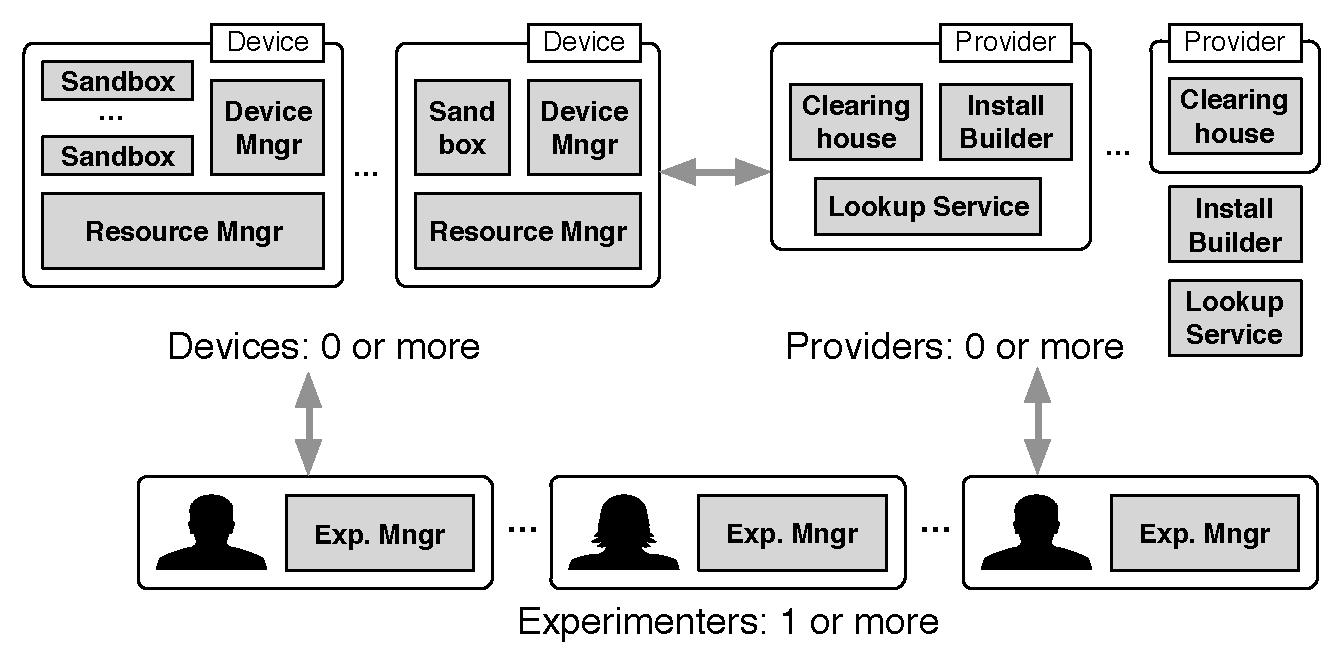
\includegraphics[width=\columnwidth]{figures/arch.pdf}
  \caption{Architecture components of Seattle}
  \label{fig:arch}
\end{figure}



Figure~\ref{fig:arch} overviews Seattle's components and interfaces.
\cite{Cappos2009} for the arch!

Sandbox: core element of computation. Self-isolating.
\cite{RepySandbox,li2015fence} for the tech!

Resource manager (nodemanager): demultiplex SB users, some SB isolation too (chroot).

Device manager (installer with \texttt{--percentage}, start/stop scripts, uninstaller, softwareupdater): device owner retains control!

Experiment manager (seash): We call user code ``experiments'' for historical reasons.

And that's it, this is an infrastructure-less deployment already!
You want more? Here you go.

Installer builder: where you get installer from; lets you plant pubkeys.

Clearinghouse: well....

Lookup service: a centralized meta-meeting point.



